\section{Results}
% Provide an introductory paragraph that summarizes what's in this section: a list of runs/experiments intended to test your implementation and ideas. Describe each of these experiments in a few words/a sentence.

In this section, we analyze how our distributed-memory implementation of the Sobel filter improves computational efficiency by leveraging parallel execution across multiple CPU nodes. We evaluate the performance of three grid decomposition strategies—Column-slab, Row-slab, and Tiled—under various concurrency levels. We start by describing the computational platform and software environment we used for our experiments. Next, we explain our methodology, including decomposition techniques, runtime measurement, data movement tracking, and speedups to assess parallel performance. Through our runtime performance and data movement studies, we identify how task distribution, communication, and synchronization influence overall efficiency. Finally, we discuss our findings and suggest optimizations to enhance scalability and performance accuracy.

\subsection{Computational platform and Software Environment}
\label{subsec:computational-platform-and-software-environment}
% What machine did you run your tests on? What was the processor, its clock rate (GHz), size of L1/L2/L3 cache, how much memory (DRAM), what OS?

% What compiler did you use, what compilation flags?

% Include a subsection describing your computational platform and software environment. Please add a citation to the location where you found this information (hint: use the LaTeX \cite{} command, and add a new entry to the template.bib file provided with the Overleaf template).

The experiments were conducted on a CPU node of the Perlmutter supercomputer at NERSC. Each node is equipped with two AMD EPYC 7763 (Milan) processors, each featuring 64 cores running at a clock rate of 2.45 GHz. These cores support Simultaneous Multi-threading (SMT), enabling two threads per core. Each core has 32 KiB of L1 cache and 512 KiB of L2 cache, while 8 cores share a 32 MiB L3 cache. The AMD EPYC 7763 processor also features 8 memory channels per socket, with 2 DIMMs per channel, and 4 NUMA domains per socket (NPS=4) \cite{amd_epyc_tuning_guide}.

The system is supported by 512 GiB of DDR4 DRAM, offering a memory bandwidth of 204.8 GiB/s per CPU. The processors utilize the AVX2 instruction set for vector processing, and each core has a peak computational throughput of 39.2 GFLOPS \cite{nersc_perlmutter_architecture}.

All experiments were conducted on a single CPU node running \textit{SUSE Linux Enterprise Server 15 SP4}, with kernel version \textit{5.14.21-150400.24.81\_12.0.87-cray\_shasta\_c} \cite{usami2024hostnamectl}. The C++ code was compiled using \textit{g++-12 (SUSE Linux) 12.3.0} with the following optimization flags: \texttt{-fopenmp -Wall -pedantic -march=native}. Note that the \texttt{-fopenmp} flag was not used for compiling the CBLAS implementation.

The following OpenMP environmental variables were used for the VMM OpenMP implementation. The variable \texttt{OMP\_NUM\_THREADS} was left unset as it conflicts with \texttt{likwid-perfctr} on Perlmutter:
\begin{itemize}
    \item \texttt{OMP\_PLACES=threads}: Assigns each OpenMP thread to a separate hardware thread, ensuring efficient mapping to processing units.
    \item \texttt{OMP\_PROC\_BIND=spread}: Distributes threads evenly across the available CPUs, aiming for optimal workload balancing.
\end{itemize}

The execution command for each program was:
\begin{quote}
\texttt{likwid-perfctr -m -g FLOPS\_DP -C N:0-\${num\_threads-1} ./benchmark -N \$N}
\end{quote}

The command runs the benchmark executable while collecting performance metrics using \texttt{likwid-perfctr}. The options used in the command are as follows:
\begin{itemize}
    \item \texttt{-g FLOPS\_DP}: Specifies the performance group to measure, in this case, the \textit{FLOPS\_DP} group, which tracks double-precision floating-point operations to evaluate computational throughput.
    \item \texttt{-C N:0-\${num\_threads-1}}: Binds the execution to a set of cores. The option \texttt{N:0-\${num\_threads-1}} allows specification of core IDs from 0 to \texttt{num\_threads-1}, where \texttt{num\_threads} represents the nuMiBer of threads being used. This ensures that only the desired cores are used during the run.
\end{itemize}
% What machine did you run your tests on? What was the processor, its clock rate (GHz), size of L1/L2/L3 cache, how much memory (DRAM), what OS?

% What compiler did you use, what compilation flags?


\subsection{Methodology}
\label{subsec:methodology}
\subsection{Methodology}
\label{subsec:methodology}

\subsubsection{Problem Sizes and Concurrency Levels}
\label{subsubsec:problem-size}
To evaluate the Sobel filter implementations, we tested a fixed grayscale image with dimensions \(7112 \times 5146\). Experiments were conducted using three decomposition methods: Row-slab, Column-slab, and Tiled. For each method, we analyzed performance across varying total ranks: 4, 9, 16, 25, 36, 49, 64, and 81, capturing the impact of concurrency on runtime.

\subsubsection{Runtime Measurement}
\label{subsubsec:runtime}
Performance data was collected by measuring the runtime of three key phases: Scatter, Sobel computation, and Gather. Timing was performed on the CPU using the C++ \texttt{chrono\_timer()}, which encapsulated the \texttt{scatterAllTiles}, \texttt{sobelAllTiles}, and \texttt{gatherAllTiles} functions, respectively. 

To ensure accurate synchronization across all ranks, \texttt{MPI\_Barrier} was employed before starting and stopping timers for each phase. This approach guarantees that all ranks finish the preceding phase before advancing to the next, thereby isolating the runtime measurements for each phase and avoiding overlap between operations.

\subsubsection{Data Movement}
\label{subsubsec:data-movement}
The number of messages and total data size were measured by implementing counters before calling \texttt{MPI\_Send} and calculating the data size using \texttt{MPI\_Type\_size}. These values were aggregated using \texttt{MPI\_Reduce} to provide a global summary.

\subsubsection{Speedup Calculation}
\label{subsubsec:speedup}
Speedup was derived from the runtime data to evaluate the parallel performance of the Sobel filter implementations. The speedup \(S(n, p)\) is defined as:

\begin{displaymath}
    S(n, p) = \frac{T^*(n)}{T(n, p)}
\end{displaymath}

Here, \(T^*(n)\) is the runtime of the best sequential algorithm for a problem of size \(n\), measured as the runtime with a single process per CPU node (total ranks of 4). \(T(n, p)\) represents the runtime for the same problem size \(n\) using \(p\) parallel threads. Since the problem size was fixed (\(7112 \times 5146\) image), the variability in \(p\) allowed us to assess the scalability of each decomposition method.

\subsection{Scaling Study for Basic OMP parallelization}
\label{subsec:scaling-study-basic}
% \begin{itemize}
%     \item Using the runtime portion of the data you collected during the performance runs, produce a speedup chart showing the scaling performance of your Basic OMP across all levels of concurrency and problem sizes in this assignment. This will be a single chart containing 3 datasets, one for each of p=4,16,64.
%     \item Discuss the performance of your Basic OMP-omp across the set of problem sizes N and concurrency levels P. Describe how speedup changes as a function of problem size, and give an explanation as to why you think that change occurs.
% \end{itemize}

% For the threads = 4 and 16, the speedup shows the steady increase nearing to the ideal speedup of 4 and 16 respectively as the matrix size N increases. According to the Amdahl's law\cite{amdahl1967validity}\footnote{Amdahl's law describes the theoretical maximum speedup that can be achieved in a parallel system based on the portion of a task that must be executed serially. The theoretical speedup limit for a problem size \(n\) and \(p\) parallel processors is given by: \( S(n, p) = \frac{1}{f + \frac{1-f}{p}} \), where \(f\) is the portion of the program that must remain serial, and \((1-f)\) is the parallelizable portion. For smaller values of \(f\), the closer the speedup is to the ideal scaling with \(p\).}, this behavior is expected because for larger matrix sizes, the overhead of the serial portion and the introduction of multithreading should be minimal. 

% For the threads = 64, N = 2048 shows the highest speedup and this is expected, however, N = 512 gives the lower speedup than N = 128 and this is unexpected. We still don't know why this happens.

% \begin{figure}
%     \centering
%     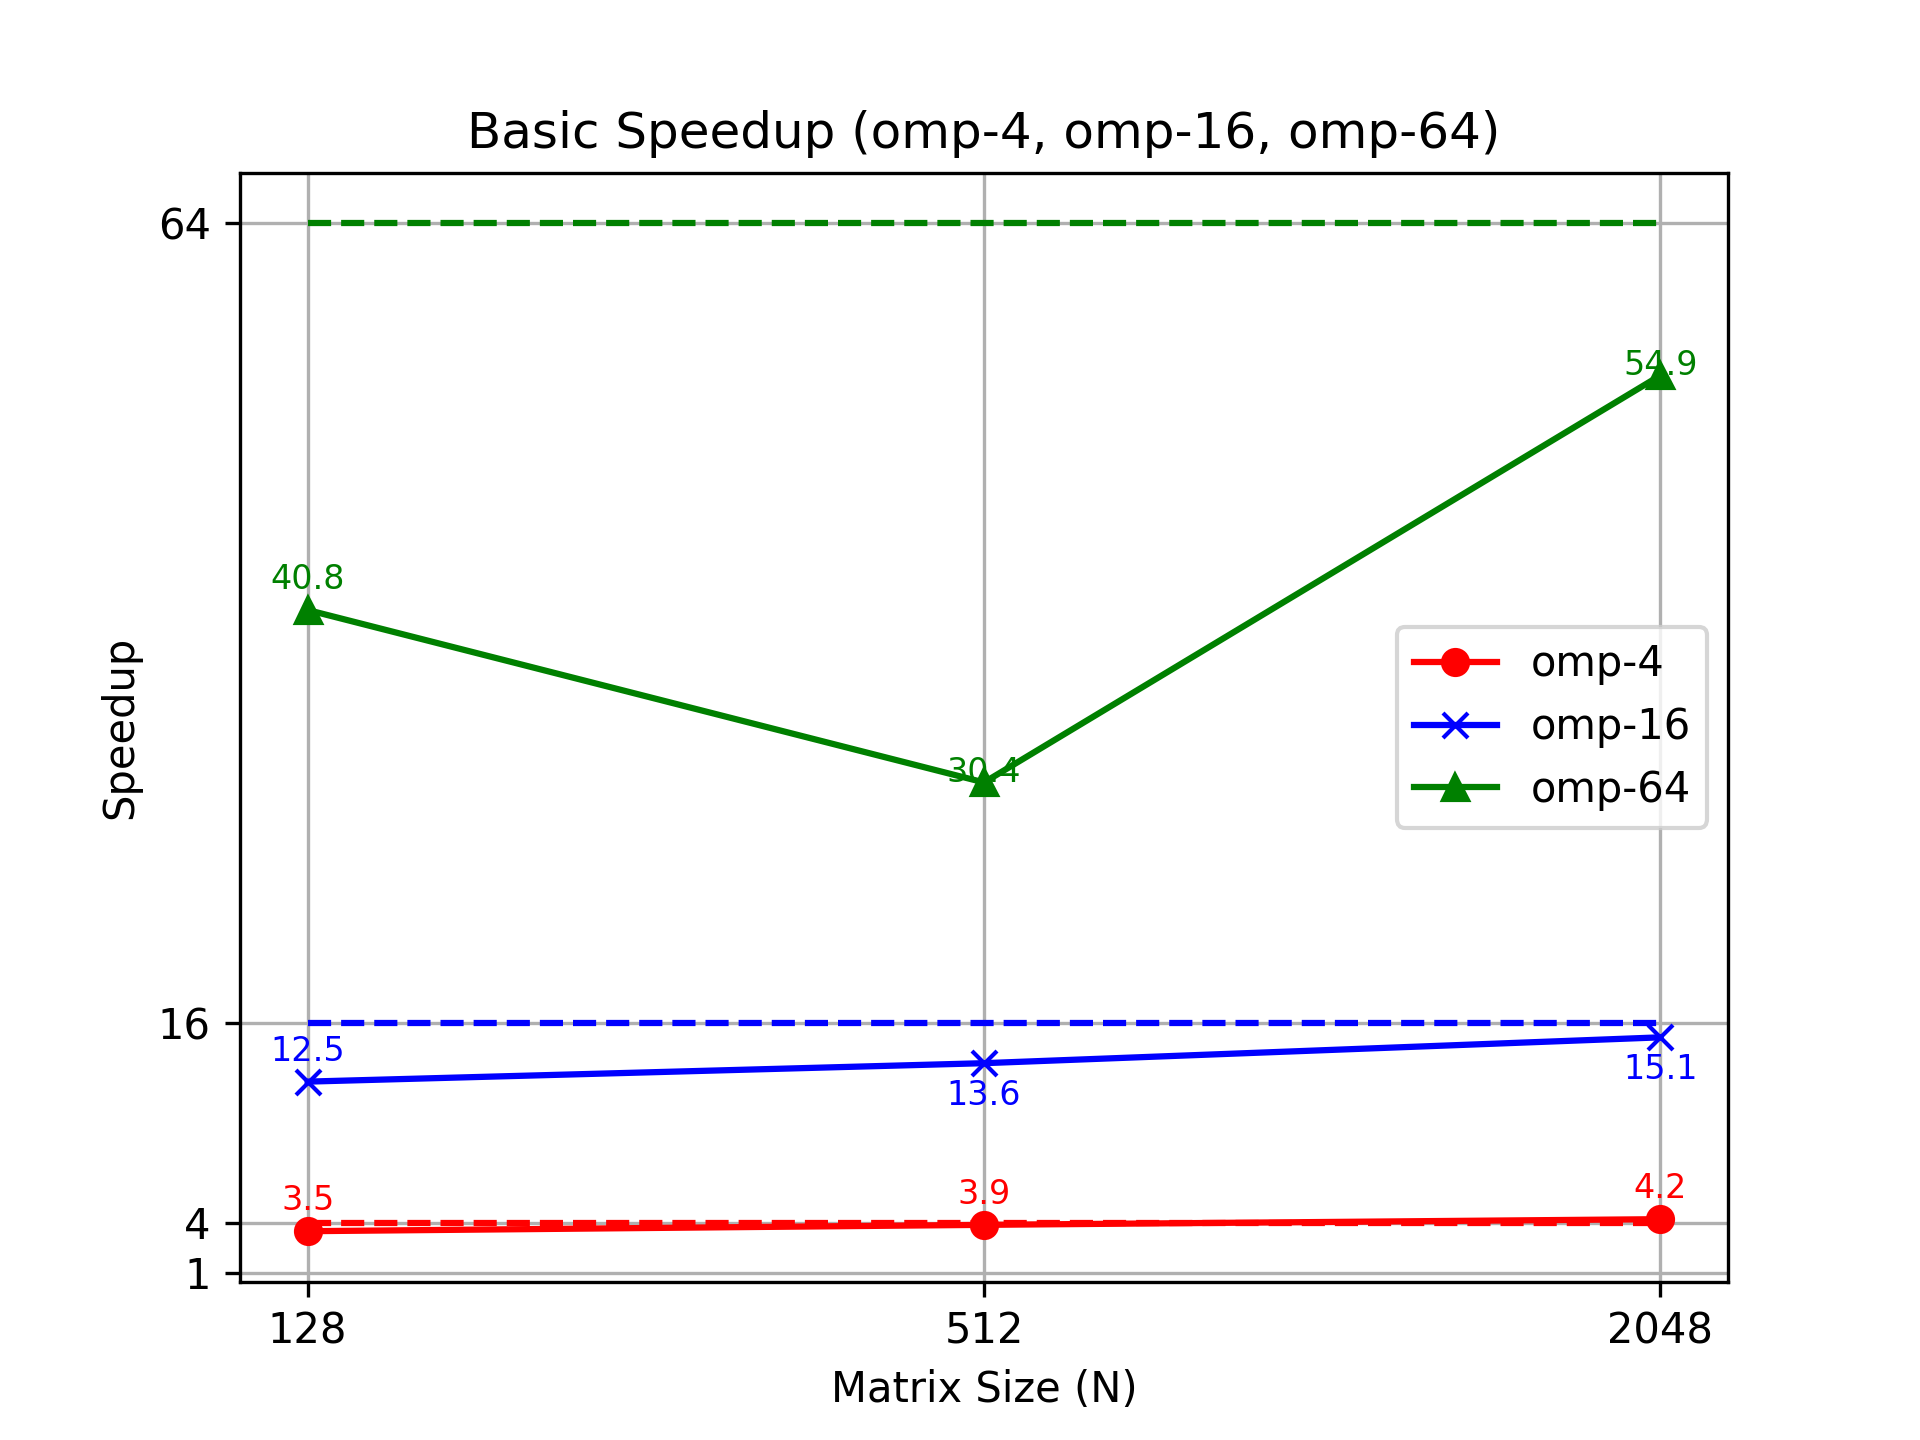
\includegraphics[width=1.0\linewidth]{images/Basic_Speedup.png}
%     \caption{Caption}
%     \label{fig:basic-speedup}
% \end{figure}

The scaling performance of the Basic OMP implementation was analyzed across different concurrency levels (\(p = 4, 16, 64\)) and matrix sizes (\(N = 128, 512, 2048\)). Figure~\ref{fig:basic-speedup} shows the speedup chart, illustrating the relationship between concurrency levels and problem sizes, allowing us to evaluate the efficiency of the parallelization approach.

For thread counts of 4 and 16, the speedup demonstrated a steady increase as the matrix size \(N\) increased, approaching the theoretical ideal speedup of 4 and 16, respectively. This behavior aligns well with expectations based on Amdahl's Law \cite{amdahl1967validity}, which suggests that for larger problem sizes, the impact of the serial portion of the code becomes less significant, thereby reducing overhead and enhancing the effectiveness of parallel execution. In other words, larger matrix sizes increase the computational workload sufficiently to minimize the negative impact of serial portions, thus leading to near-ideal speedup values.

For a thread count of 64, the results were somewhat mixed. The highest speedup was observed for \(N = 2048\), which was expected given the increased computational workload and better utilization of the available cores. However, an unexpected observation was made for \(N = 512\), where the speedup was lower compared to \(N = 128\). This deviation requires further investigation.

\begin{figure}[htbp]
    \centering
    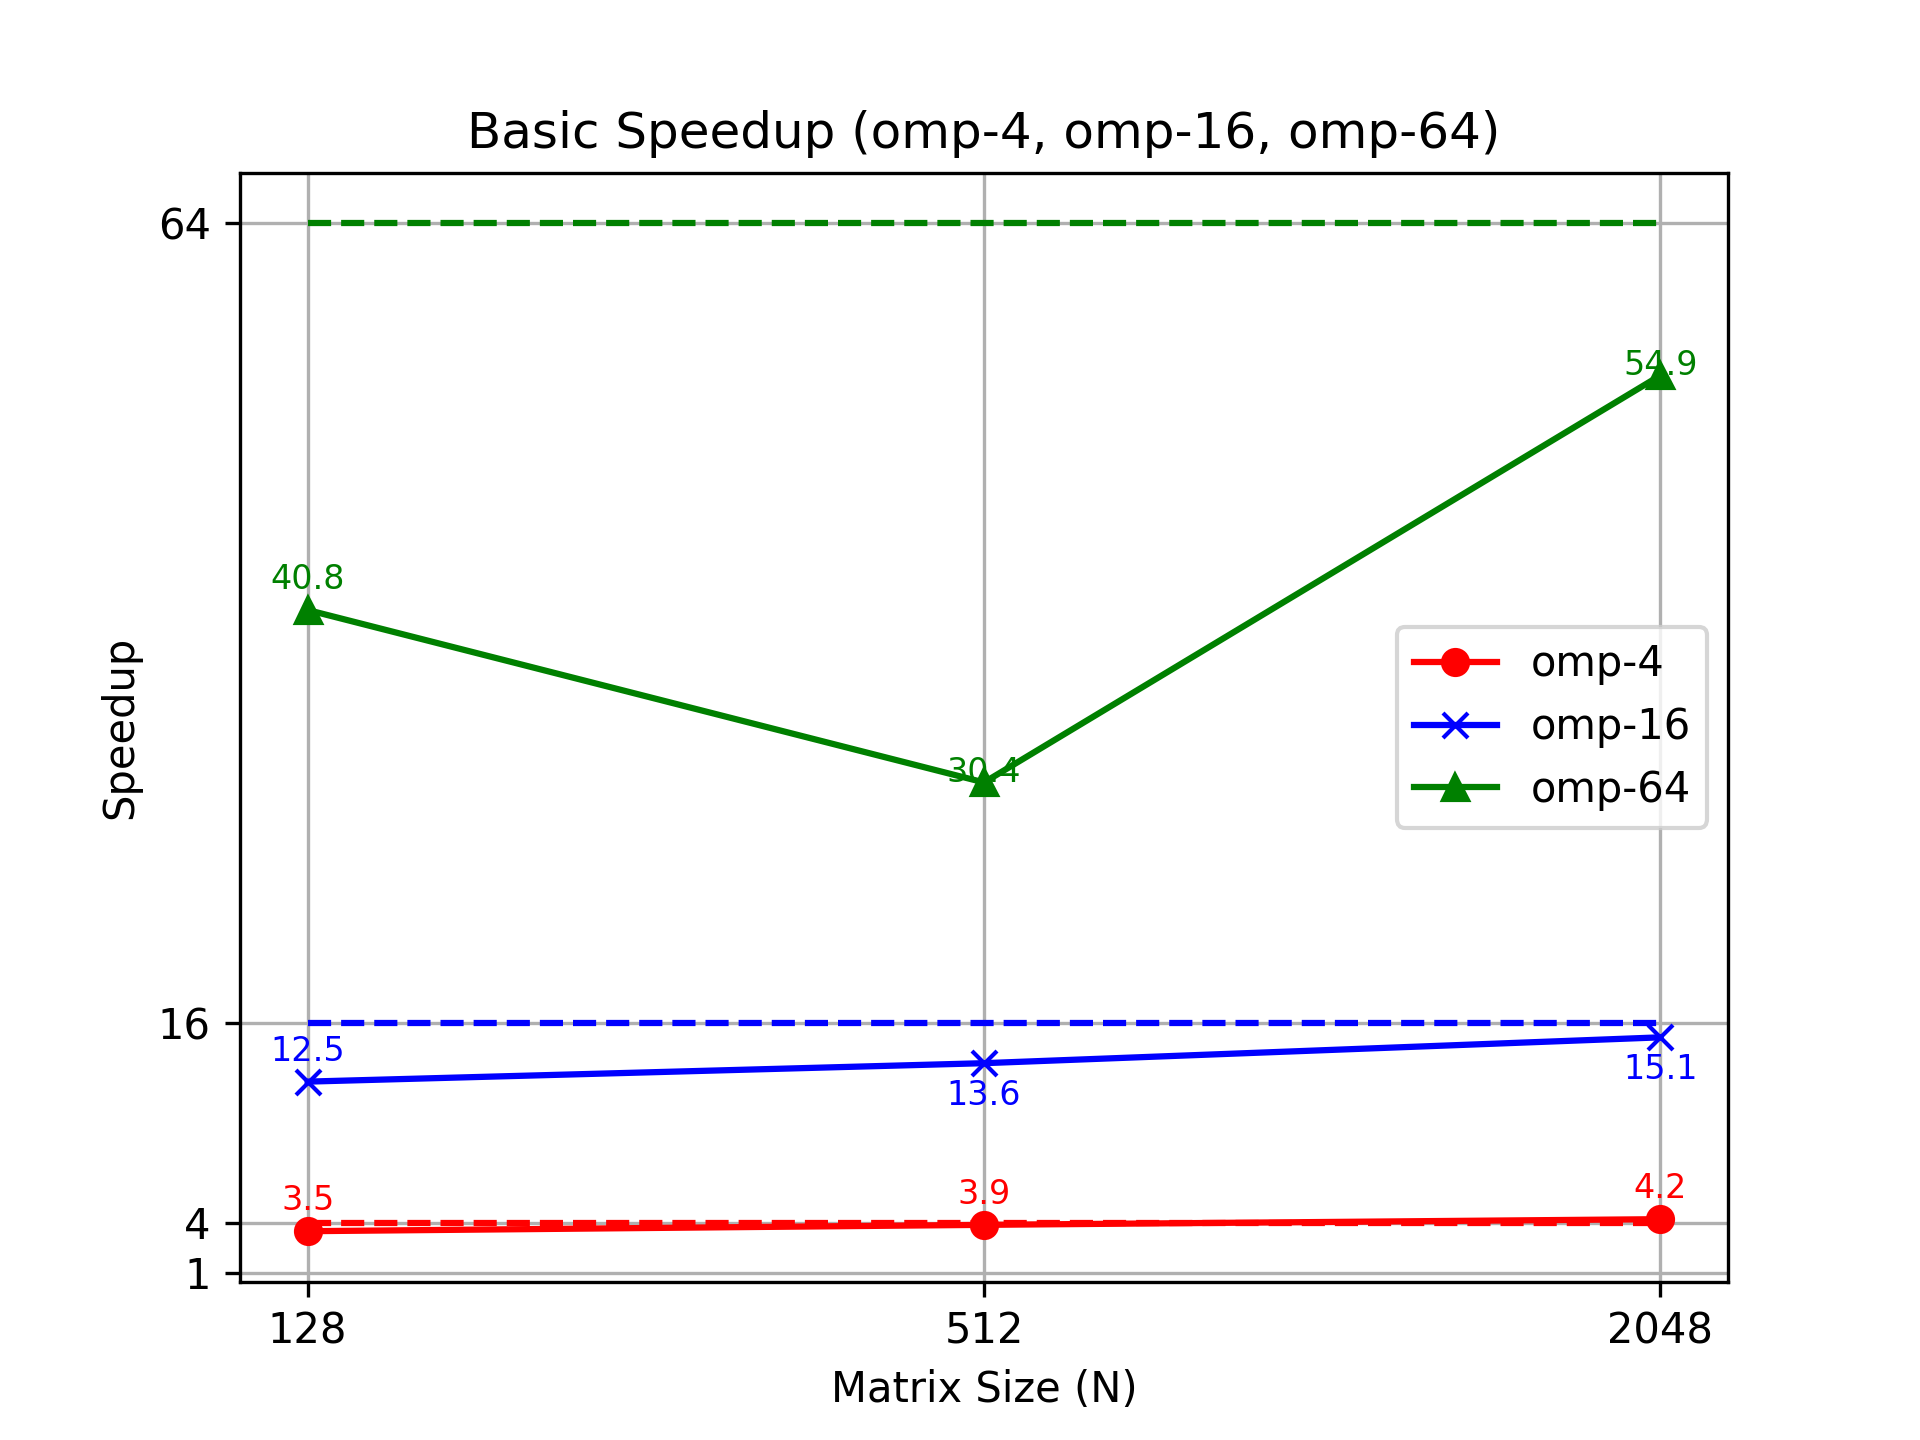
\includegraphics[width=1.0\linewidth]{images/Basic_Speedup.png}
    \caption{\textbf{Speedup of Basic OMP with OpenMP Parallelization.} The figure shows the speedup achieved by the Basic OMP implementation at different concurrency levels (\(p = 4, 16, 64\)) for matrix sizes of \(N = 128, 512, 2048\). The ideal speedup for each concurrency level is also shown for comparison, highlighting the efficiency of parallelization as the matrix size increases. It is observed that for \(p = 64\), the speedup for \(N = 512\) is unexpectedly lower compared to \(N = 128\), suggesting potential issues such as cache contention or memory bandwidth limitations.}
    \label{fig:basic-speedup}
\end{figure}

Interestingly, when measuring runtime using \texttt{std::chrono::high\_resolution\_clock}, as shown in Figure~\ref{fig:basic-speedup-chrono}, the results appear more consistent with the expected outcomes of Amdahl's Law. Specifically, for each thread count, \(N = 128\) consistently achieves lower speedup, while larger \(N\) values yield speedup results that are closer to the theoretical ideal. This steady increase in speedup as \(N\) increases suggests that the instrumentation code used in Listing~\ref{listing:measuring-elapsed-time} provides a more accurate representation of the expected scaling behavior.

\begin{figure}[htbp]
    \centering
    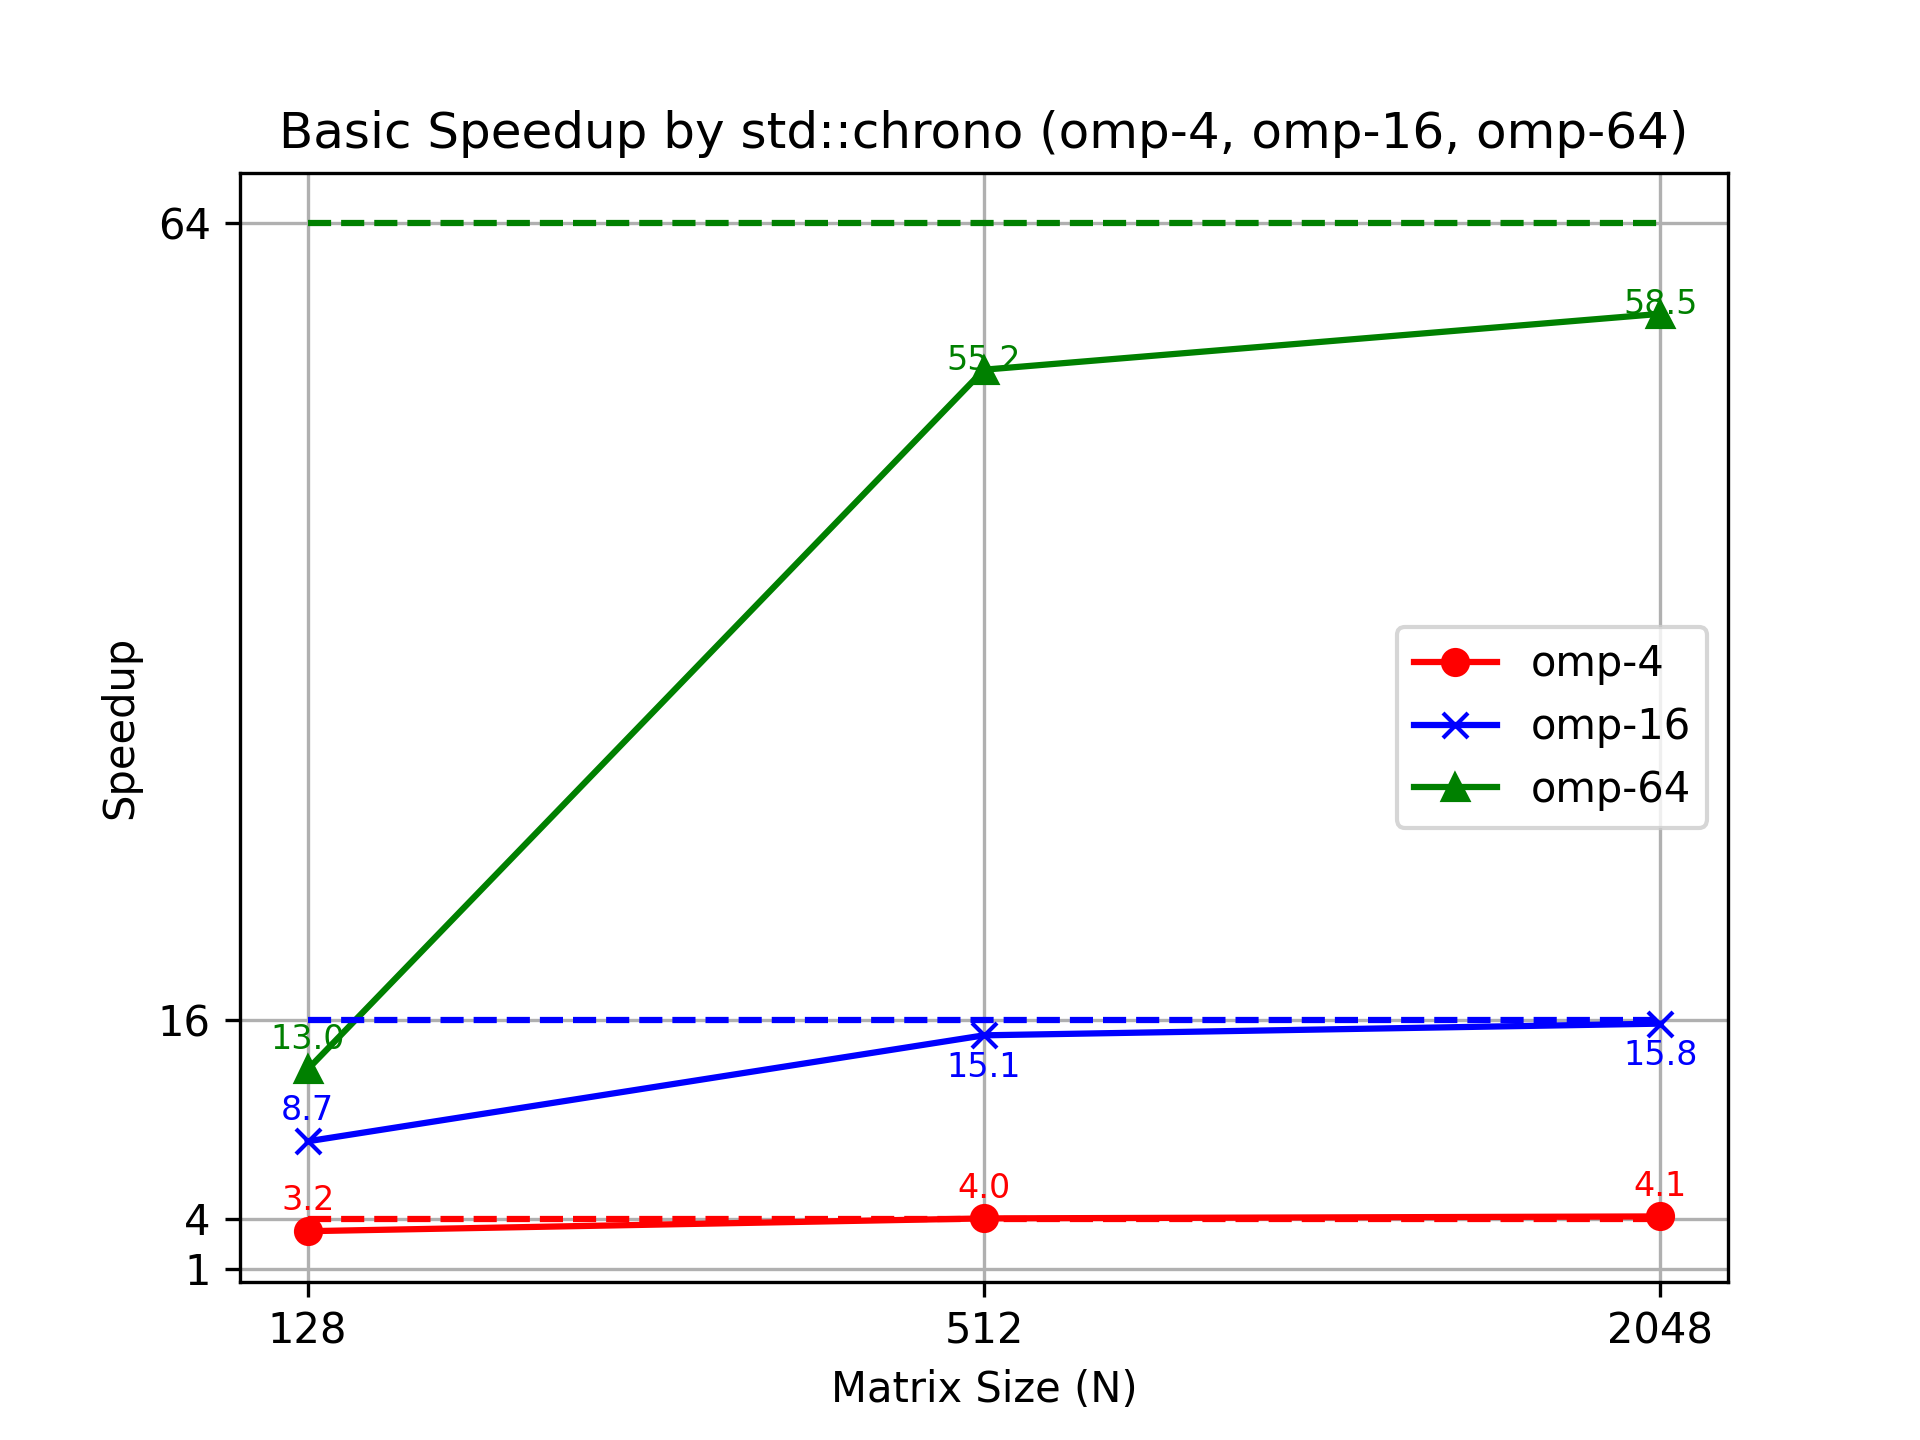
\includegraphics[width=1.0\linewidth]{images/Basic_Speedup_chrono.png}
    \caption{\textbf{Speedup of Basic OMP with OpenMP Parallelization measured by std::chrono::high\_resolution\_clock.} This figure shows the speedup results when using \texttt{std::chrono::high\_resolution\_clock} for measuring elapsed time. Unlike the previous measurements, the speedup values exhibit more predictable scaling behavior, consistent with Amdahl's Law, where larger matrix sizes (\(N = 512\), \(N = 2048\)) result in improved speedup, while \(N = 128\) demonstrates lower efficiency.}
    \label{fig:basic-speedup-chrono}
\end{figure}

\begin{lstlisting}[caption={Instrumentation code for measuring the elapsed time of MM},label={listing:measuring-elapsed-time},name=measuring-elapsed-time,float=htbp,style=mystyle,language=C++]
setup(n, A, B, C);
start_time = get_high_resolution_clock_now();
square_dgemm(n, A, B, C);
end_time = get_high_resolution_clock_now();
elapsed_time = end_time - start_time;
\end{lstlisting}

\FloatBarrier
\subsection{Evaluation of BMMCO OMP parallelization}
% \begin{itemize}
%     \item Using the runtime portion of the data you collected during the performance runs, produce a speedup chart showing the scaling performance of your BMMCO-omp code across all levels of concurrency and problem sizes in this assignment. This will be a single chart containing 6 datasets: three concurrency levels,  t=4,16,64, and two block sizes, b=4,16.
%     \item Discuss the performance of your BMMCO-omp code across the set of problem sizes, block sizes, and concurrency levels. Describe how speedup changes as a function of problem size, and give an explanation as to why you think that change occurs. 
% \end{itemize}

The scaling performance of the BMMCO OMP implementation was analyzed across different concurrency levels (\(p = 4, 16, 64\)), block sizes (\(b = 4, 16\)), and matrix sizes (\(N = 128, 512, 2048\)). Figure~\ref{fig:blocked-speedup} presents the speedup chart for six different configurations, illustrating the interplay between concurrency levels, block sizes, and problem sizes.

Overall, the scaling behavior aligns well with Amdahl's Law \cite{amdahl1967validity}, with larger matrix sizes yielding near-ideal speedup as parallelism increases. Larger problem sizes effectively reduce the overhead from serial portions of the code and allow for more efficient workload distribution across threads.

One notable observation is that a block size of 4 achieved better speedup for smaller matrix sizes (\(N = 128, 512\)) compared to a block size of 16. Specifically, Blocked B16 at concurrency levels of \(p = 16, 64\) for \(N = 128\) and \(p = 64\) for \(N = 512\) exhibited limited speedup. Additionally, Blocked B4 for \(N = 128\) showed that increasing the thread count from \(p = 16\) to \(p = 64\) actually resulted in worse performance. These observations can be attributed to how parallelism was applied in the BMMCO implementation, where the outermost loop was parallelized (as shown in Listing~\ref{listing:BMMCO-omp}). The number of iterations in this outermost loop corresponds to the number of blocks along a row, which directly affects thread utilization.

Tables~\ref{tab:b4-threads-utilization} and \ref{tab:b16-threads-utilization} show the number of blocks per row for different matrix sizes and block sizes, along with the corresponding thread utilization for different concurrency levels. For \(b = 16\) and \(N = 128\), only 8 blocks are available, which limits the number of threads that can be effectively utilized to 8. This is significantly lower than the total available threads for configurations with \(p = 16, 64\), leading to underutilization of potential parallelism. Similarly, for \(N = 512\), \(b = 16\) results in 32 blocks, which limits effective thread utilization to 32 when using \(p = 64\).

On the other hand, \(b = 4\) provides more blocks for each problem size, which enables better thread utilization, particularly for smaller matrices like \(N = 128\). For \(N = 128\), \(b = 4\) allows for 32 blocks, which is sufficient to fully utilize threads for configurations with \(p = 4, 16\). However, increasing the thread count to \(p = 64\) resulted in underutilization, as the overhead of multithreading outweighed the performance gain from adding more threads. 

In conclusion, block size has a significant impact on scaling performance, particularly for smaller problem sizes. The availability of sufficient blocks to match the number of threads determines the efficiency of parallelism. For larger matrices (\(N = 2048\)), both block sizes showed good scalability, as there were enough blocks available to fully utilize all threads across all concurrency levels.

\begin{figure}[htbp]
    \centering
    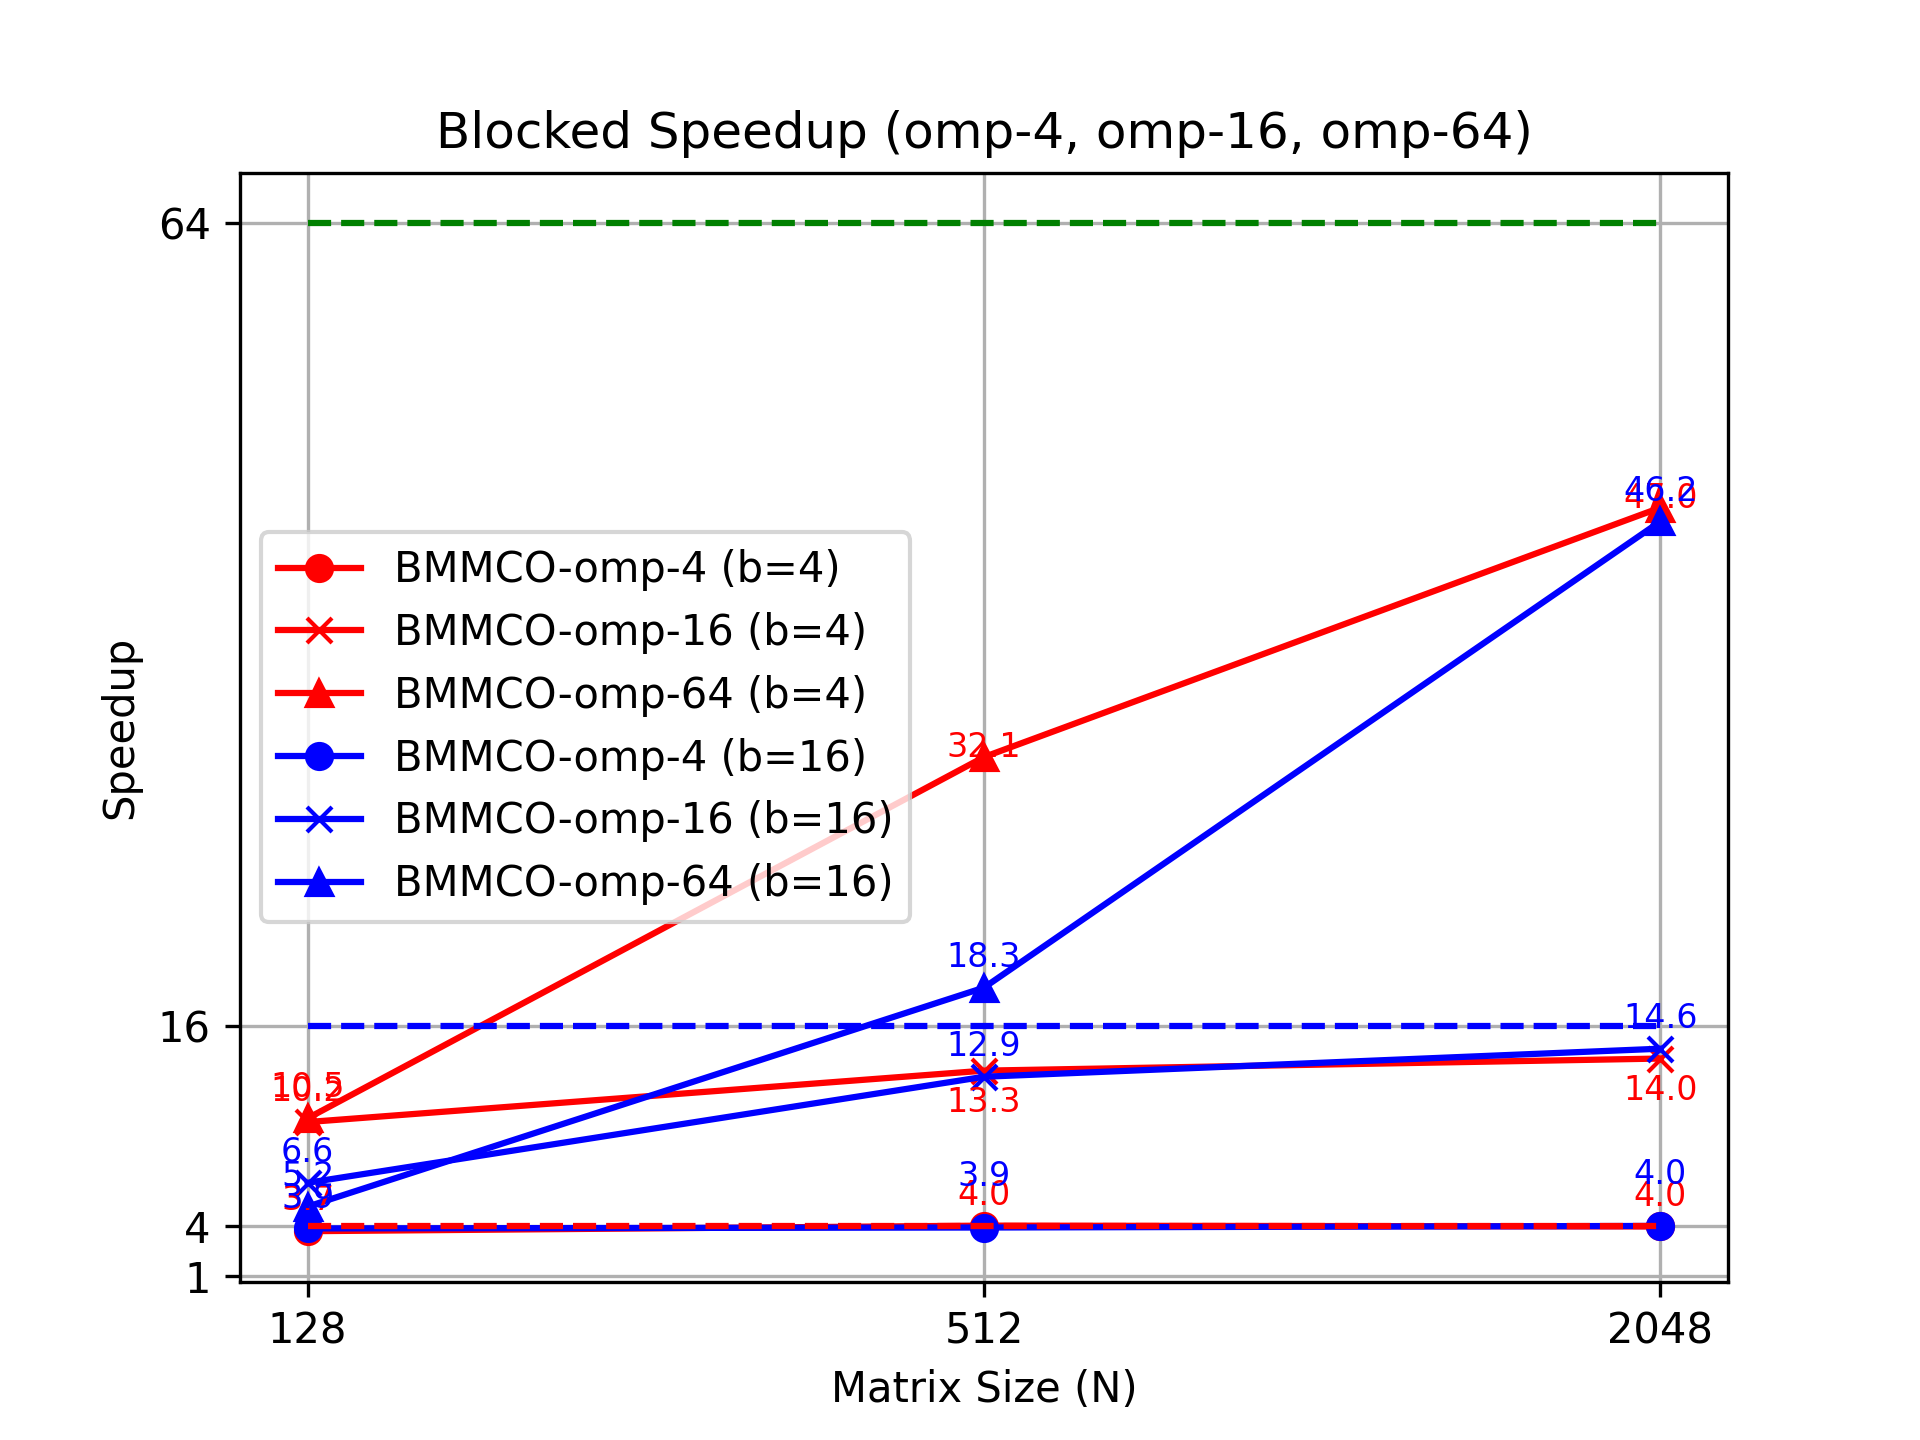
\includegraphics[width=1.0\linewidth]{images/Blocked_Speedup.png}
    \caption{\textbf{Speedup of BMMCO with OpenMP Parallelization for Different Block Sizes.} The figure shows the speedup achieved by the BMMCO implementation at different concurrency levels (\(p = 4, 16, 64\)) for matrix sizes of \(N = 128, 512, 2048\) with block sizes of \(b = 4\) and \(b = 16\). The results demonstrate that \(b = 4\) generally provides better performance for smaller matrix sizes due to improved thread utilization, whereas \(b = 16\) struggles to fully leverage available threads for smaller matrices.}
    \label{fig:blocked-speedup}
\end{figure}

\begin{table}[htbp]
    \centering
    \begin{tabular}{lrrrr}
    \toprule
    N & Blocks & \(p=4\) & \(p=16\) & \(p=64\) \\
    \midrule
    128  & 32 & 100\% & 100\% & 50\% \\
    512  & 128 & 100\% & 100\% & 100\% \\
    2048 & 512 & 100\% & 100\% & 100\% \\
    \bottomrule
    \end{tabular}
    \caption{\textbf{Number of Blocks per Row and Thread Utilization for Block Size of 4.} The table shows the number of blocks per row for different matrix sizes and the resulting thread utilization percentage for different concurrency levels. Block size \(b = 4\) provides sufficient blocks to maintain high thread utilization for most configurations.}
    \label{tab:b4-threads-utilization}
\end{table}

\begin{table}[htbp]
    \centering
    \begin{tabular}{lrrrr}
    \toprule
    N & Blocks & \(p=4\) & \(p=16\) & \(p=64\) \\
    \midrule
    128  & 8 & 100\% & 50\% & 12.5\% \\
    512  & 32 & 100\% & 100\% & 50\% \\
    2048 & 128 & 100\% & 100\% & 100\% \\
    \bottomrule
    \end{tabular}
    \caption{\textbf{Number of Blocks per Row and Thread Utilization for Block Size of 16.} The table shows the number of blocks per row for different matrix sizes and the resulting thread utilization percentage for different concurrency levels. Block size \(b = 16\) results in fewer blocks for smaller matrices, which limits the effective thread utilization, particularly at higher concurrency levels.}
    \label{tab:b16-threads-utilization}
\end{table}


\FloatBarrier
\subsection{Comparison of CBLAS, Basic OMP, and BMMCO OMP}
\label{subsec:comparison-cblas-basic-bmmco}
\subsubsection{L1 Cache Utilization}
\label{subsubsec:memory-hierarchy-utilization-l2}
    % \item Question: looking at data in this table, what observations do you make about the relative number of L2 Accesses being made by each code? How do you reason these values might affect runtime?

L2 accesses represent the number of requests that are not satisfied by the L1 cache and, therefore, must be handled by the L2 cache. The Basic implementation shows L2 accesses that are between 50 and 100 times greater than those for CBLAS, indicating significantly poorer cache efficiency. In contrast, Blocked B4 has L2 accesses roughly 5 to 8 times higher than CBLAS, indicating an improvement compared to Basic but still relatively far from optimal. Blocked B16, with L2 accesses between 1.2 and 1.8 times that of CBLAS, demonstrates the closest behavior to the highly optimized CBLAS implementation.

These results indicate that Blocked B16 achieves the most efficient use of the L2 cache, as its L2 access values are closest to those of CBLAS, which serves as the baseline for an optimized memory access pattern. Increasing the block size from 4 to 16 leads to a significant reduction in L2 accesses, highlighting the impact of larger block sizes in enhancing data locality and reducing the need for higher-level cache accesses.

It is reasonable to assume that the runtime of these methods is proportional to the number of L2 accesses, given that the number of floating-point operations (FLOPs) remains largely consistent across implementations. Therefore, the primary factor contributing to runtime differences is the efficiency of memory access patterns and cache utilization. The reduced L2 cache accesses observed in the blocked methods, particularly Blocked B16, should contribute to lower runtimes compared to Basic OMP, as fewer requests to higher levels of the memory hierarchy result in fewer latency penalties.

\begin{table}[htbp]
    \centering
    \begin{tabular}{lrrrr}
    \toprule
    N &  CBLAS &  Basic &  Blocked B4 &  Blocked B16 \\
    \midrule
    128  &      1 &  47.89&       5.37&         1.19\\
    512  &      1 &  45.53&       4.41&         1.30\\
    2048 &      1 & 116.14&       7.91&         1.86\\
    \bottomrule
    \end{tabular}
    \caption{\textbf{L2 Cache accesses.} The table shows the value of the L2 Accesses metric normalized by the corresponding value of the L2 Accesses metric for CBLAS. Blocked B4 refers to the blocked method with a block size of 4, and Blocked B16 refers to the blocked method with a block size of 16. The CBLAS column serves as a baseline with all values equal to 1, while the other columns represent the ratio of L2 accesses compared to CBLAS for each problem size. Basic OMP shows significantly higher L2 accesses compared to CBLAS, whereas Blocked B16 achieves the closest values to CBLAS, indicating more efficient cache usage and better alignment with an optimized memory access pattern.}
    \label{tab:l2-cache}
\end{table}

\FloatBarrier
\subsubsection{L2 Cache Utilization}
\label{subsubsec:memory-hierarchy-utilization-l3}
% \item Question: looking at data in this table, what observations do you make about the relative number of L3\_CACHE\_REQ being made by each code? How do you reason these values might affect runtime?

L3\_CACHE\_REQ represents the number of requests that are not satisfied by the L2 cache and, therefore, must be handled by the L3 cache. For larger matrix sizes (\(N = 512\) and \(N = 2048\)), the Basic implementation exhibits an order of magnitude more L3 cache requests compared to the blocked methods, indicating inefficient L2 cache utilization. Blocked B16 consistently demonstrates approximately 5 to 6 times fewer L3 cache requests than Blocked B4, suggesting that increasing the block size significantly improves data locality and cache efficiency, thus reducing the dependency on L3 cache. 

Interestingly, for \(N = 128\), Basic, Blocked B4, and Blocked B16 show fewer L3 cache requests than CBLAS. This suggests some overhead in the CBLAS implementation that necessitates additional L3 cache accesses.

We assume that the runtime of these methods is closely correlated to the number of L3 cache requests, as the number of FLOPs required for MM remains relatively constant across implementations. Therefore, the primary factor contributing to runtime differences is the efficiency of memory access patterns and cache utilization. The significant reduction in L3 cache requests observed in the blocked methods, particularly Blocked B16, likely translates to lower runtimes compared to Basic OMP due to fewer accesses to higher memory levels and the associated lower latency penalties.

\begin{table}[htbp]
    \centering
    \begin{tabular}{lrrrr}
    \toprule
    N &  CBLAS &  Basic &  Blocked B4 &  Blocked B16 \\
    \midrule
    128  &      1 &  0.41 &       0.44 &         0.60 \\
    512  &      1 & 283.96 &      18.51 &         3.61 \\
    2048 &      1 & 578.74 &      22.49 &         4.16 \\
    \bottomrule
    \end{tabular}
    \caption{\textbf{L3 Cache accesses.} The table shows the value of the L3\_CACHE\_REQ counter normalized to the corresponding value for CBLAS. The CBLAS column contains values of 1, serving as a baseline, while the other columns represent the ratio of L3 cache requests relative to CBLAS for each problem size. Blocked B4 refers to the blocked method with a block size of 4, and Blocked B16 refers to the blocked method with a block size of 16. For larger matrix sizes (\(N = 512, 2048\)), Basic OMP shows significantly higher L3 cache requests compared to CBLAS, whereas Blocked B16 achieves values closest to CBLAS, indicating more efficient L3 cache usage. However, for \(N = 128\), Basic, Blocked B4, and Blocked B16 show fewer requests than CBLAS, suggesting an overhead in CBLAS that increases L3 access.}
    \label{tab:l3-cache}
\end{table}

\begin{table}[htbp]
    \centering
    \begin{tabular}{lccccc}
    \toprule
    N &  CBLAS &  Basic &  Blocked B4 &  Blocked B16 & L2 \\
    \midrule
    128  & 384 KiB & 384 KiB & 384 KiB & 390 KiB & Yes \\
    512  & 6 MiB   & 6 MiB   & 6 MiB   & 6 MiB   & No  \\
    2048 & 96 MiB  & 96 MiB  & 96 MiB  & 96 MiB  & No  \\
    \bottomrule
    \end{tabular}
    \caption{\textbf{Memory Footprint for Different Matrix Sizes and Methods.} The table shows the memory required for matrices of each size and whether they fit within the L2 cache (512 KiB). Each method requires memory for three matrices. In addition, the blocked methods require three blocks, which are relatively small except for Blocked B16 at \(N = 128\).}
    \label{tab:memory-footprint}
\end{table}


\FloatBarrier
\subsubsection{Instruction count analysis: RETIRED\_INSTRUCTIONS}
\label{subsubsec:instruction-count}
% \item Question: looking at the values in this table, please provide observations and reasoning about:
% \begin{itemize}
%     \item The relative number of instructions being executed compared to CBLAS.
%     \item How do you reason these differences might impact code performance?
%     \item What difference do you see in the blocked B4 and B16 codes? How do you reason about their meaning and their potential impact on performance?
% \end{itemize}

The relative number of instructions executed compared to CBLAS is approximately 10 times greater for Basic, 24 to 28 times for Blocked B4, and 12 to 13 times for Blocked B16. In the case of Basic, the increased instruction count does not significantly impact runtime since the primary bottleneck lies in memory access rather than arithmetic operations. This is indicative of Basic's poor cache utilization and frequent memory accesses.

For the blocked methods, however, memory access is significantly optimized, which makes the number of retired instructions more directly proportional to runtime. The larger instruction counts for Blocked B4 compared to Blocked B16 suggest inefficiencies that could be linked to fewer vectorization opportunities or less efficient use of fused multiply-add (FMA) instructions. Blocked B16, with a lower instruction count than Blocked B4, indicates more efficient execution likely due to better cache locality and greater potential for hardware-level optimizations such as vectorization and FMA usage. As such, the reduced instruction count in Blocked B16 can contribute to improved runtime performance.

\begin{table}[htbp]
    \centering
    \begin{tabular}{lrrrr}
    \toprule
    N &  CBLAS &  Basic &  Blocked B4 &  Blocked B16 \\
    \midrule
    128  &      1 &  9.99 &      24.66 &         11.88 \\
    512  &      1 & 10.60 &      27.48 &         13.28 \\
    2048 &      1 & 10.64 &      27.74 &         13.42 \\
    \bottomrule
    \end{tabular}
    \caption{\textbf{Instruction Count Analysis.} The table shows the RETIRED\_INSTRUCTIONS counter values normalized by the corresponding value for CBLAS, with CBLAS values set to 1 as a baseline. The relative instruction counts for Basic, Blocked B4, and Blocked B16 provide insights into the efficiency of different implementations. Basic OMP has significantly higher instruction counts compared to CBLAS, while Blocked B16 shows lower instruction counts than Blocked B4, indicating more efficient execution due to better optimization techniques.}
    \label{tab:instruction-count}
\end{table}

\FloatBarrier
\subsection{Findings and Discussion}
\label{subsec:findings-and-discussion}
% \begin{itemize}
%     \item Scaling characteristics of basic and blocked codes. Looking at your two speedup charts, what observations do you make about the relative scalability of these three codes: basic, blocked B4 and blocked B16? What are limits to scalability? How might you modify the codes to reduce the impact of those limitations? 
%     \item Comments about memory system utilization. Looking across the data in Tables 1 and 2 (L2CACHE, L3CACHE), what observations to you make about how well, or not, each of the 4 codes (CBLAS, basic-serial, blocked B4 serial, blocked B16 serial) makes use of the memory system hierarchy? Be clear in your description what you mean by “makes use of the memory system hierarchy” and use data from the Tables to validate your statements.
% \end{itemize}
Overall, Basic OMP scaled well as the level of parallelism increased, particularly due to the large number of iterations in the outermost loop. However, for BMMCO, particularly when the matrix size was small and the block size large, the performance gains from parallelism were limited due to underutilization of threads. In these cases, the number of blocks per row was insufficient to fully leverage the available threads. To mitigate this limitation, we could modify the code by collapsing two outermost loops, increasing the effective number of iterations and thus improving thread utilization.

As shown in Table~\ref{tab:l2-cache} and Table~\ref{tab:l3-cache}, Basic OMP exhibits poor cache utilization, particularly for L1 and L2 caches, when compared to CBLAS. Blocked B16 demonstrates much better L1 cache utilization, approaching the efficiency of CBLAS (only 1.2x to 1.8x more L2 accesses). However, Blocked B16 is still not fully utilizing the L2 cache, as its L3 requests are 3.6x to 4.2x those of CBLAS for larger matrix sizes. Blocked B4 falls between Basic OMP and Blocked B16 in terms of cache efficiency, showing moderate improvement over Basic OMP but still trailing behind Blocked B16 in terms of L1 and L2 cache utilization.

To improve memory system utilization for the blocked methods, increasing the block size helps reduce the number of higher-level cache accesses, but we need to balance this against the number of available blocks and their impact on parallel thread utilization. An optimal balance between block size and parallelism can significantly reduce latency penalties from memory hierarchy inefficiencies, leading to better overall performance.


\begin{comment}
%% the material that follows is from the generic tech paper skeleton project


How our solution performed, how its performance compared to that of other solutions mentioned in related work, and how these results show that our solution is effective
\begin{itemize}
    \item Presentation and Interpretation
    \item Why, how, and to what degree our solution is better
    \item Why the reader should be impressed with our solution
    \item Comments
    \item Here is a cross reference to Table~\ref{tab:my_label} and Fig.~\ref{fig:my_label}.
\end{itemize}

Context and limitations of our solution as required for summation
\begin{itemize}
    \item What the results do and do not say
\end{itemize}

\end{comment}